\section{ HÀM SỐ BẬC HAI}
\subsection{TÓM TẮT LÝ THUYẾT}

\subsubsection{Hàm số bậc hai $y=ax^2+bx+c$, với $a \ne 0$.}
\begin{itemize}
	\item[\ding{172}] Tập xác định $\mathbb{R}$.
	\item [\ding{173}] Tọa độ đỉnh $S\left(-\dfrac{b}{2a};-\dfrac{\Delta}{4a} \right)$. \textit{Để xác định nhanh tọa độ đỉnh, ta chỉ cần xác định hoành độ $x_0$. Sau đó thay $x_0$ vào hàm số, ta tính $y_0$}.
	\item [\ding{174}] Sự biến thiên của hàm số bậc hai:\\
	\begin{minipage}[b]{7cm}
		\begin{khung4}{$a>0$}
			
\begin{tikzpicture}
				\tkzTabInit[lgt=1,espcl=2]
				{$x$/1,$y$/2}
				{$-\infty$,$-\dfrac{b}{2a}$,$+\infty$}
				\tkzTabVar{+/$+\infty$,-/$-\dfrac{\Delta}{4a}$,+/$+\infty$}
			\end{tikzpicture}
			\begin{itemize}
				\item $a>0$ thì bề lõm quay lên.
				\item Hàm số nghịch biến trên $\left(-\infty;-\frac{b}{2a} \right)$; đồng biến trên $\left(-\frac{b}{2a};+\infty \right)$.
			\end{itemize}
		\end{khung4}
	\end{minipage}\hspace{1cm}
	\begin{minipage}[b]{7cm}
		\begin{khung4}{$a<0$}
			
\begin{tikzpicture}
				\tkzTabInit[lgt=1,espcl=2]
				{$x$/1,$y$/2}
				{$-\infty$,$-\dfrac{b}{2a}$,$+\infty$}
				\tkzTabVar{-/$-\infty$,+/$-\dfrac{\Delta}{4a}$,-/$-\infty$}
			\end{tikzpicture}
			\begin{itemize}
				\item $a<0$ thì bề lõm quay xuống.
				\item Hàm số đồng biến trên $\left(-\infty;-\frac{b}{2a} \right)$; nghịch biến trên $\left(-\frac{b}{2a};+\infty \right)$.
			\end{itemize}
		\end{khung4}
	\end{minipage}
\end{itemize}

\subsubsection{Đồ thị hàm số bậc hai $y=ax^2+bx+c$, với $a \ne 0$.}

\begin{itemize}
	\item [\ding{172}] Trong mặt phẳng $Oxy$, đồ thị là một parabol:\\
	\hspace*{1cm}
	\begin{tikzpicture}[smooth,samples=300,scale=0.6,>=stealth]
		\draw[->] (-0.8,0)--(4.5,0) node[below]{$x$};
		\draw[->] (0,-1.5)--(0,2.5) node[right]{$y$};
		\draw (0,0) node[above left]{$O$};
		\draw[thick, magenta,domain=0.3:3.7] plot(\x,{(\x)^2-4*(\x)+3});
		\draw[fill=blue] (2,-1) circle(1.5pt) (2,0) circle(1pt) (0,-1) circle(1pt);
		\draw[dashed] (2,-1.5)--(2,2.5) (2,-1)--(0,-1)node[left]{\footnotesize$-\dfrac{\Delta}{4a}$};
		\node[right] at (2,2.4) {\footnotesize $x=-\tfrac{b}{2a}$};
		\node[right] at (0.5,-2) {\fbox{\footnotesize$a>0$}};
	\end{tikzpicture}
	\hspace*{4cm}
	\begin{tikzpicture}[smooth,samples=300,scale=0.6,>=stealth]
		\draw[->] (-0.8,0)--(4.5,0) node[below]{$x$};
		\draw[->] (0,-1.5)--(0,2.5) node[right]{$y$};
		\draw (0,0) node[above left]{$O$};
		\draw[thick, magenta,domain=0.2:3.8] plot(\x,{-(\x)^2+4*(\x)-2});
		\draw[fill=blue] (2,2) circle(1.5pt) (2,0) circle(1pt) (0,2) circle(1pt);
		\draw[dashed] (2,-1.4)--(2,2.5) (2,2)--(0,2)node[left]{\footnotesize$-\dfrac{\Delta}{4a}$};
		\node[right] at (2,-1.5) {\footnotesize $x=-\tfrac{b}{2a}$};
		\node[right] at (0.5,-2) {\fbox{\footnotesize$a<0$}};
	\end{tikzpicture}
	\item [\ding{173}] Trục đối xứng: $x=-\dfrac{b}{2a}$ (\textit{xem đồ thị}).
	\item [\ding{174}] Cắt trục tung tại điểm có tung độ bằng $c$, tức là đồ thị luôn qua điểm $(0;c)$.
	\item [\ding{175}] Giá trị lớn nhất (max), giá trị nhỏ nhất (min)
	\begin{itemize}
		\item Khi $a>0$, hàm số đạt \textbf{giá trị nhỏ nhất} $y_{\min} =-\dfrac{\Delta}{4a}$ khi $x=-\dfrac{b}{2a}$ (tại đỉnh).
		\item Khi $a<0$, hàm số đạt \textbf{giá trị lớn nhất} $y_{\max} =-\dfrac{\Delta}{4a}$ khi $x=-\dfrac{b}{2a}$ (tại đỉnh).
	\end{itemize}
\end{itemize}

\subsection{RÈN LUYỆN KĨ NĂNG GIẢI TOÁN}
\begin{dang}{Đồ thị hàm số bậc hai và các vấn đề liên quan}
	\indamm{Muốn vẽ parabol, ta cần là các bước sau:}
	\begin{listEX}[1]
		\item [\ding{172}] Xác định tọa độ đỉnh $S(x_0;y_0)$, với $x_0=-\dfrac{b}{2a}$, $y_0$ được tính bằng cách thay $x_0$ vào hàm số và bấm máy.
		\item [\ding{173}] Xác định trục đối xứng $d \colon x=-\dfrac{b}{2a}$.
		\item [\ding{174}] Lập bảng giá trị (5 điểm), hoặc tìm giao điểm với $Ox$, $Oy$.
		\item [\ding{175}] Xác định "chiều quay" của parabol và vẽ \indamm{parabol} có đỉnh $S$, có trục đối xứng $d$ và qua các điểm vừa xác định. 
	\end{listEX}
\end{dang}

\begin{vd}
	Vẽ đồ thị và xác định tập giá trị của các hàm số sau đây
	\begin{listEX}[3]
		\item $y=2x^2$.
		\item $y=x^2-4x+1$.
		\item $y=-x^2-2x+3$.
		\item $y=-x^2-2$.
		\item $y=-\dfrac{1}{4}x^2+\dfrac{3}{2}x+\dfrac{7}{4}$.
		\item $y=\dfrac{2}{3}x^2-\dfrac{4}{3}x+2$.
	\end{listEX}
	\loigiai{}
\end{vd}
\begin{vd}%[0D2Y3]
	Cho hàm số $y=-x^2-3x+1$ có đồ thị là parabol $(P)$. 
	\begin{tasks}(1)
		\task Tìm tọa độ của đỉnh, giao điểm của đồ thị $(P)$ với trục tung và trục hoành.
		\task Tìm các khoảng đồng biến và nghịch biến của hàm số.
	\end{tasks}
		\loigiai{}
\end{vd}
\begin{vd}%[0D2Y3]
	Cho hàm số $y=x^2-4x+3$ có đồ thị là parabol $(P)$. 
	\begin{tasks}
		\task Tìm các khoảng đồng biến và nghịch biến của hàm số. 
		\task Vẽ đồ thị $(P)$.
	\end{tasks}
	\loigiai{}
\end{vd}

\begin{dang}{Xác định hàm số bậc hai $y=ax^2+bx+c$}
	Việc xác định $(P)$ hay đi tìm các hệ số $a$, $b$, $c$, ta thường quy về việc giải hệ phương trình liên quan đến ba ẩn  $a$, $b$, $c$. Khi tìm các phương trình liên quan, ta chú ý một số nội dung sau:
	\begin{itemize}
		\item[\iconMT] Nếu đề cho $(P)$ qua điểm $(x_0;y_0)$ thì ta được: $ax_0^2+bx_0+c=y_0$.
		\item[\iconMT] Nếu đề cho tọa độ đỉnh là $(x_0;y_0)$ thì ta được
		\begin{listEX}[1]
			\item [\ding{172}] Hoành độ đỉnh $-\dfrac{b}{2a}=x_0$;
			\item [\ding{173}] $(x_0;y_0) \in (P)$, suy ra $ax_0^2+bx_0+c=y_0$.
			\item [\ding{174}] $(P)$ viết dưới dạng $y=a(x-x_0)^2+y_0$.
		\end{listEX}
		\item[\iconMT] Nếu đề cho hoành độ đỉnh (hoặc trục đối xứng) $x=x_0$, ta được $-\dfrac{b}{2a}=x_0$.
		\item[\iconMT] Nếu đề cho tung độ đỉnh $y=y_0$, ta được $-\dfrac{\Delta}{4a}=y_0$.
	\end{itemize}
\end{dang}
\begin{vd}
	Xác định phương trình của $(P)\colon y=-2x^2+bx+c$, biết
	\begin{tasks}
		\task $(P)$ đi qua hai điểm $M(0;-2)$ và $N(2;0)$;
		\task $(P)$ có đỉnh $I(1;3)$;
		\task $(P)$ đi qua điểm $A(2;-3)$ và có hoành độ đỉnh $x_0=3$;
		\task $(P)$ có trục đối xứng là $x=2$ và cắt trục hoành tại điểm có hoành độ bằng $2$.
	\end{tasks}
	\loigiai{}
\end{vd}

\begin{vd}
	Xác định hàm số $y=ax^2+bx+c$ có đồ thị $(P)$, biết 
	\begin{tasks}
		\task $(P)$ đi qua ba điểm $A(1;0)$, $B(2;8)$ và $C(0;-6)$.
		\task $(P)$ đi qua điểm $A(0;5)$ và có đỉnh $I(3;-4)$.
		\task Hàm số đạt giá trị nhỏ nhất bằng $3$ và đồ thị $(P)$ qua các điểm $(0;5)$, $(3;13)$.
	\end{tasks}
	\loigiai{}
\end{vd}

\begin{vd}
	Hãy viết phương trình của parabol ứng với mỗi đồ thị dưới đây.
	\begin{listEX}[2]
		\item \begin{tikzpicture}[smooth,samples=300,scale=0.5,>=stealth]
			\draw[->] (-7,0)--(2,0) node[above]{$x$};
			\draw[->] (0,-5)--(0,1.5) node[right]{$y$};
			\draw (0,0) node[above left]{$O$};
			\draw[domain=-6.3:0.35] plot(\x,{-4/9*(\x)^2-8/3*(\x)-4});
			\draw[fill=black] (-3,0) circle(1.5pt) (0,-4) circle(1.5pt);
			\draw[dashed] (-3,0)--(-3,-4.7);
			\node[above] at (-3,0) {\small $-3$};
			\node[right] at (0,-4) {\small $-4$};
		\end{tikzpicture}
		\item \begin{tikzpicture}[smooth,samples=300,scale=0.8,>=stealth]
			\draw[->] (-4,0)--(2,0) node[below]{$x$};
			\draw[->] (0,-1.5)--(0,2) node[right]{$y$};
			\draw (0,0) node[above left]{$O$};
			\draw[domain=-3.5:1.5] plot(\x,{4/9*(\x)^2+8/9*(\x)-5/9});
			\draw[fill=black] (-1,-1) circle(1.5pt) (0.5,0) circle(1.5pt) (-1,0) circle(1pt) (0,-1) circle(1pt);
			\draw[dashed] (0,-1)--(-1,-1)--(-1,2);
			\node[left] at (0,-1.3) {\small $-1$};
			\node[above] at (-1.3,0) {\small $-1$};
			\node[below] at (0.7,0) {\small $\dfrac{1}{2}$};
		\end{tikzpicture}
	\end{listEX}
	\loigiai{}
\end{vd}


\begin{dang}{Ứng dụng của hàm số bậc hai trong thực tế}
	\begin{itemize}
		\item [\iconMT] Một số mô hình thực tế (cổng chào, cầu,...) có hình dạng parabol;
		\item [\iconMT] Một số chuyển động có phương trình quỹ đạo là một hàm bậc hai.
	\end{itemize}
	Khi thực hiện đo đạc tính toán, ta thường dùng lý thuyết về hàm số bậc hai để giải các bài toán trên.
\end{dang}

\begin{vd}%[0D2T3]
	Một vật chuyển động với vận tốc $v=40+18t-t^2$ (m/s). Trong $20$ giây đầu vận tốc lớn nhất của vật là bao nhiêu?\\
	\hspace*{2cm} \boxminit{Đáp số: $v_{\max}=121$ m/s.}
	\loigiai{
		\immini{Đồ thị của hàm vận tốc $v$ có dạng Parabol  bề lõm hướng xuống dưới. Đỉnh của Parabol là $I(9;121)$. Do đó trong đoạn $[0;20]$, vận tốc lớn nhất của vật là $121$ m/s.
		}{
			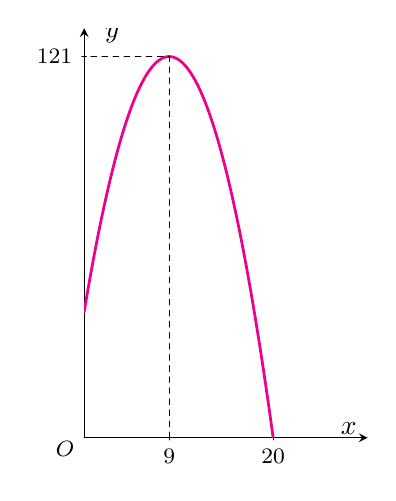
\begin{tikzpicture}[line cap=round,line join=round,>=stealth,x=0.3cm,y=0.1cm, scale=0.4]
				\draw[->,color=black] (0,0.) -- (30,0.);
				\foreach \x in {9,20}
				\draw[shift={(\x,0)},color=black] (0pt,2pt) -- (0pt,-2pt) node[below] {\footnotesize $\x$};
				\draw[->,color=black] (0.,0) -- (0.,130);
				\foreach \y in {121}
				\draw[shift={(0,\y)},color=black] (2pt,0pt) -- (-2pt,0pt) node[left] {\footnotesize $\y$};
				\draw[color=black] (0pt,-10pt) node[left] {\footnotesize $O$};
				\clip(0,0) rectangle (30,130);
				\draw[line width=1pt,color=magenta,smooth,samples=100,domain=0:20] plot(\x,{40+18*\x-(\x)^2});
				\draw [dash pattern=on 2pt off 2pt] (9,0)--(9,121)--(0,121);
				\draw (28, 3)  node {$x$}; \draw (3,128)  node {$y$};
			\end{tikzpicture}
	}}
\end{vd}

\begin{vd}%[0D2T3]
	\immini{Cổng vào miền Tây (Gateway Arch) ở thành phố St. Louis, nước Mỹ, có hình dạng là một phần của parabol như hình vẽ. Khoảng cách giữa 2 chân cổng $AB=160\,\mathrm{m}$. Trên thành cổng, tại vị trí có độ cao $45\,\mathrm{m}$ so với mặt đất (tại điểm $M$), người ta thả một sợi dây chạm đất (dây căng thẳng theo phương vuông góc với đất). Vị trí chạm đất của đầu sợi dây này cách chân cổng $A$ một đoạn $10\,\mathrm{m}$. Hãy tính khoảng cách từ mặt đất đến điểm cao nhất của cổng.\\
		\hspace*{2cm} \boxminit{Đáp số: $192$ m}
	}
	{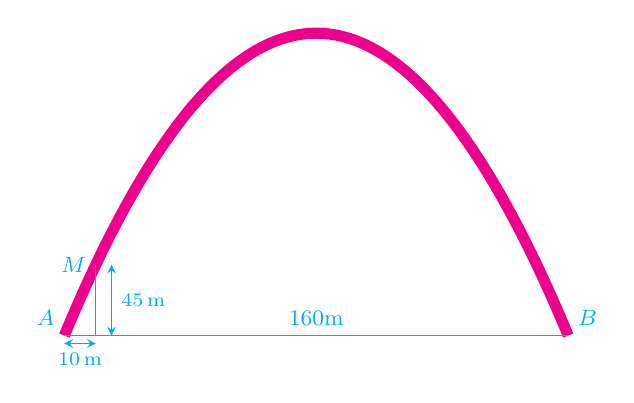
\begin{tikzpicture}[scale=0.2,>=stealth,x=2mm,y=1mm]
			\draw[line width=4pt,magenta,smooth,samples=100,domain=0:160,/pgf/fpu,/pgf/fpu/output format=fixed] plot(\x,{-0.03*(\x)^2+4.8*(\x)});
			\draw[cyan] (0,0) node[above left] {\footnotesize $A$} -- (80,0)node[above] {\footnotesize $160$m}--(160,0) node[above right]{\footnotesize $B$} (10,45) node[left]{\footnotesize $M$};
			\draw[cyan](10,0)--(10,45);
			\draw[<->,thin,cyan](15,0)--(15,45) node[midway,right]{\scriptsize $45\,\mathrm{m}$};
			\draw[<->,thin,cyan] (0,-5)--(10,-5) node[midway,below]{\scriptsize $10\,\mathrm{m}$};
			\usepgflibrary{fpu}
		\end{tikzpicture}
	}
	\loigiai{
		\immini{Đặt hệ trục toạ độ với $Axy$ như hình vẽ.\\
			Xét parabol $(P):\,y=ax^2+bx+c$.\\
			$M\in(P)\Leftrightarrow100a+10b+c=45$\\
			$A\in(P)\Leftrightarrow c=0$. $B\in(P)\Leftrightarrow160^2a+160b+c=0$.\\
			Giải hệ được $y=-0,03x^2+4,8x$.\\
			$\Rightarrow$ Chiều cao cổng là $y(80)=192\,\mathrm{m}$.
		}
		{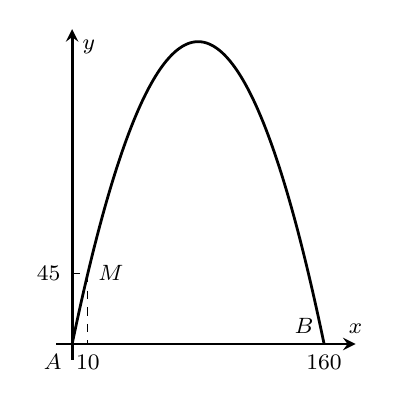
\begin{tikzpicture}[scale=0.2,line width=1pt,>=stealth,x=1mm,y=1mm]
				\draw (0,0) node[below left] {\footnotesize $A$} (10,45) node[right]{\footnotesize $M$} (160,0) node[above left]{\footnotesize $B$};
				\draw[->] (-10,0) -- (180,0) node [above] {\footnotesize$x$};
				\draw[->] (0,-10) -- (0,200) node [below right] {\footnotesize$y$};
				\foreach \x/\xtext in {10/10,160/160}
				\draw[shift={(\x,0)}] (0pt,2pt)--(0pt,-2pt) node[below] {\footnotesize $\xtext$};
				\foreach \y/\ytext in {45/45}
				\draw[shift={(0,\y)}] (2pt,0pt)--(-2pt,0pt) node[left] {\footnotesize $\ytext$};
				\draw[dashed,thin] (0,45)--(10,45)--(10,0);
				\usepgflibrary{fpu}
				\draw[smooth,samples=100,domain=0:160,/pgf/fpu,/pgf/fpu/output format=fixed] plot(\x,{-0.03*(\x)^2+4.8*(\x)});
			\end{tikzpicture}
		}
	}
\end{vd}

\begin{vd}%[0D2T3]
	\immini{
		Một chiếc cổng hình Parabol bao gồm một cửa chính hình chữ nhật ở giữa và hai cánh cửa phụ hai bên như hình vẽ. Biết chiều cao cổng Parabol là $4$ m còn kích thước cửa ở giữa là $3$ m $\times$ $4$ m. Hãy tính khoảng cách giữa hai điểm $A$ và $B$. (xem hình minh họa bên).\\
		\hspace*{2cm} \boxminit{Đáp số: $AB=8$}
	}
	{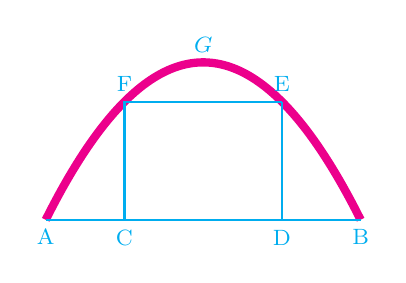
\begin{tikzpicture}[scale=0.5,thick,>=stealth,font=\footnotesize,cyan]
			\draw[line width=3pt,magenta,smooth,samples=100,domain=-4:4] plot(\x,{-0.25*(\x)^2});
			\draw[dashed,thin](2,-1)node[above]{ E};
			\draw[dashed,thin](-2,-1)node[above]{F};
			\draw[dashed,thin](-4,-4)node[below]{ A};
			\draw[dashed,thin](4,-4)node[below]{B};
			\draw[thick](2,-1)--(-2,-1)--(-2,-4)node[below]{ C}--(2,-4)node[below]{D}--(2,-1);
			\draw[thick](-4,-4)--(4,-4);
			\draw (0,0) node[above] { $G$};
		\end{tikzpicture}
	}
	\loigiai
	{\immini{Chọn hệ trục tọa độ $Oxy$ như hình vẽ với $O\equiv G$.\\Gọi phương trình của parabol là $y=ax^2+bx+c, a\neq 0$.\\Do parabol đi qua gốc tọa độ $O$ nên $c=0$.\\Do parabol có trục đối xứng $x=0$ nên $b=0\Rightarrow (P): y=ax^2$.\\Do kích thước cửa ở giữa là $3$ m $\times$ $4$ m và chiều cao cổng parabol là $4$ m nên $OI=4$ m, $HI=3$ m, $CD=4$ m $\Rightarrow HE=2$ m, $OH=1$ m $\Rightarrow E(2;-1)$ và $B\left(x_B; -4\right)$ với $x_B>0$.\\Do $E\in (P)$ nên tìm được $a=-\dfrac{1}{4}\Rightarrow (P): y=-\dfrac{1}{4}x^2$.\\Do $B\in (P)$ nên tìm được $x_B=4$. Vậy $AB=8$ m.}
		{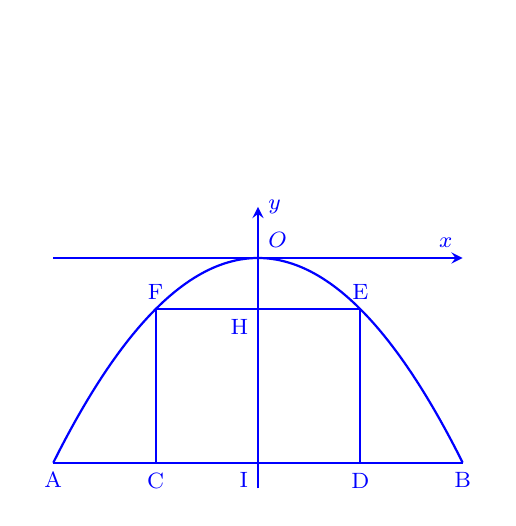
\begin{tikzpicture}[scale=0.65,thick,>=stealth,blue]
				\draw[->] (-4,0) -- (4,0) node [above left] {\footnotesize $x$};
				\draw[->] (0,-4.5) -- (0,1) node [right] {\footnotesize $y$};
				\draw[dashed,thin](2,-1)node[above]{\footnotesize E};
				\draw[dashed,thin](0,-1)node[below left]{\footnotesize H};
				\draw[dashed,thin](0,-4)node[below left]{\footnotesize I};
				\draw[dashed,thin](-2,-1)node[above]{\footnotesize F};
				\draw[dashed,thin](-4,-4)node[below]{\footnotesize A};
				\draw[dashed,thin](4,-4)node[below]{\footnotesize B};
				\draw[thick](2,-1)--(-2,-1)--(-2,-4)node[below]{\footnotesize C}--(2,-4)node[below]{\footnotesize D}--(2,-1);
				\draw[thick](-4,-4)--(4,-4);
				\draw (0,0) node[above right] {\footnotesize $O$};
				\clip (-4.5,-4.5) rectangle (4.5,4.5);
				\draw[smooth,samples=100,domain=-4:4] plot(\x,{-0.25*(\x)^2});
			\end{tikzpicture}
		}
	}
\end{vd}

\begin{vd}%[0D2T3-5]
	Khi quả bóng được đá lên, nó sẽ đạt độ cao nào đó rồi rơi xuống đất. Biết rằng quỹ đạo của quả bóng là một cung parabol trong mặt phẳng với hệ tọa độ $Oth$, trong đó $t$ là thời gian (tính bằng giây), kể từ khi quả bóng được đá lên; $h$ là độ cao (tính bằng mét) của quả bóng. Giả thiết rằng quả bóng được đá lên từ độ cao $1{,}2$ m. Sau đó $1$ giây, nó đạt độ cao $8{,}5$ m và $2$ giây sau khi đá lên, nó ở độ cao $6$ m. Hãy tìm hàm số bậc hai biểu thị độ cao $h$ theo thời gian $t$ và có phần đồ thị trùng với quỹ đạo của quả bóng trong tình huống trên.\\
	\hspace*{2cm} \boxminit{Đáp số: $h=-4{,}9t^2 + 12{,}2t + 1{,}2$}
	\loigiai
	{
		Gọi $h=at^2+bt+c$ ($a\neq 0$).\\
		Chọn mốc thời gian $t=0$ tại thời điểm quả bóng được đá lên từ độ cao $1{,}2$ m, suy ra $c=1{,}2$. Do đó biểu thức của $h$ có dạng $h=at^2+bt+1{,}2$ ($a\neq 0$).\\
		Tại thời điểm $t=1$ giây nó đạt độ cao $8{,}5$ m nên ta có $a+b=7{,}3$.\\
		Tại thời điểm $t=2$ giây nó đạt độ cao $6$ m nên ta có $4a+2b=4{,}8$.\\
		Như vậy ta có
		\begin{eqnarray*}
			\left\{\begin{aligned}&a+b=7{,}3 \\&4a+2b=4{,}8\end{aligned}\right. \Leftrightarrow \left\{\begin{aligned}&a=-4{,}9 \\&b=12{,}2.  \end{aligned}\right.
		\end{eqnarray*}
		Vậy $h=-4{,}9t^2 + 12{,}2t + 1{,}2$.
	}
\end{vd} 

\begin{vd}%[0D2T3-5]
	Chiếc cầu dây văng một nhịp được thiết kế hai bên thành cầu có dạng parabol và được cố định bằng các dây cáp song song.
	\begin{center}
		\begin{tikzpicture}[scale=0.3, font=\footnotesize, line join=round, line cap=round, >=stealth]
			\tikzset{thanh-cau/.pic={
					\draw[scale=0.3,smooth, samples=100, domain=-15:15] plot (\x,{(7/375)*(\x)^2+0.8});
					\foreach \i in {-1.5,-3,-4.5,-6,-7.5,-9,-10.5,-12,-13.5,-15,0,1.5,3,4.5,6,7.5,9,10.5,12,13.5,15} \draw[scale=0.3] (\i,0)--(\i,{(4.2/225)*(\i)^2+0.8});
					\draw[scale=0.3] (-15,0)--(15,0);
			}}
			\path (0,0)pic{thanh-cau};
			\draw [color=gray,fill=cyan!40] (-15,0)--(15,0)--(13,-2)--(-17,-2)--cycle;
			\path (-2,-2)pic{thanh-cau};
			\draw (0,-3.3) node{Hình vẽ cầu dây văng};
			
		\end{tikzpicture}\\
		\vspace{1 cm}
		\begin{tikzpicture}[scale=0.3, font=\footnotesize, line join=round, line cap=round, >=stealth]
			\tikzset{thanh-cau/.pic={
					\draw[scale=0.3,smooth, samples=100, domain=-15:15] plot (\x,{(7/375)*(\x)^2+0.8});
					\foreach \i in {-1.5,-3,-4.5,-6,-7.5,-9,-10.5,-12,-13.5,-15,0,1.5,3,4.5,6,7.5,9,10.5,12,13.5,15} \draw[scale=0.3] (\i,0)--(\i,{(4.2/225)*(\i)^2+0.8});
					\draw[scale=0.3] (-15,0)--(15,0);
			}}
			\path (0,0)pic{thanh-cau};
			\draw[blue,<->] (-15,-0.5)--(15,-0.5);
			\draw[blue,<->] (15.5,0)--(15.5,5);
			\draw[blue,<->] (-15.5,0)--(-15.5,5);
			\draw (15.5,2.5) node[right]{$5$ m};
			\draw (-15.5,2.5) node[left]{$5$ m};
			\draw (0,-0.5) node[below]{$30$ m};
			\draw[<-] (0,0.4)--(2,2) node[above]{$0{,}8$ m};
			\draw (0,-3) node{Hình chiếu đứng của cầu dây văng};
			
		\end{tikzpicture}
	\end{center}
	Dựa vào bản vẽ ở hình bên, hãy tính chiều dài tổng cộng của các dây cáp dọc ở hai mặt bên. Biết
	\begin{itemize}
		\item[] Dây dài nhất là $5$ m, dây ngắn nhất là $0{,}8$ m, khoảng cách giữa các dây bằng nhau.
		\item[] Nhịp cầu dài $30$ m.
		\item[] Cần tính thêm $5$\% chiều dài mỗi sợi dây cáp để neo cố định.
	\end{itemize}
	\hspace*{2cm} \boxminit{Đáp số: $103{,}2$ m}
	\loigiai{
		Chọn hệ trục tọa độ sao cho đầu mút $A$ của dây ngắn nhất thuộc trục tung và thanh ngang mặt cầu thuộc trục hoành. Gọi $B$ là điểm đầu mút bên phải (khi nhìn thẳng vào mặt bên của thành cầu) của dây cáp dài nhất thì với các giả thiết:
		\begin{itemize}
			\item Dây dài nhất là $5$ m, dây ngắn nhất là $0{,}8$ m. Khoảng cách giữa các dây bằng nhau.
			\item Nhịp cầu dài $30$ m.
		\end{itemize}
		Ngoài ra, từ bản vẽ ta thấy có tất cả $21$ dây cáp dọc. Suy ra $A(0;0{,}8)$, $B(15;5)$.\\
		Do parabol nhận trục tung là trục đối xứng nên hàm số có công thức $y=f(x)=ax^2+c$.\\
		Ta tìm được $a=\dfrac{4{,}2}{225}$ và $c=0{,}8$. Như vậy $y=\dfrac{4{,}2}{225}x^2+0{,}8$.
		\begin{center}
			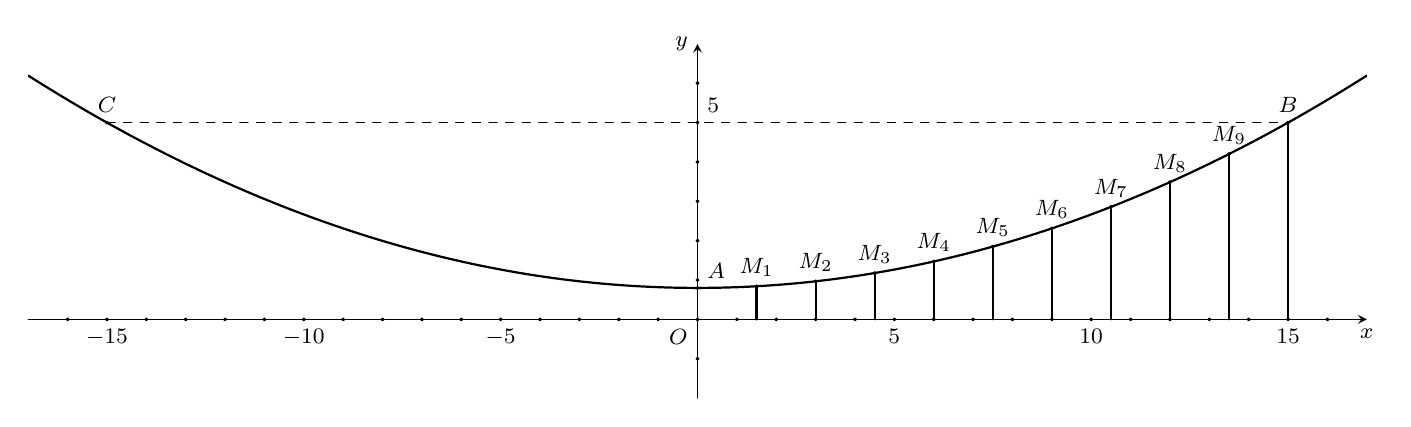
\begin{tikzpicture}[scale=0.5, font=\footnotesize, line join=round, line cap=round, >=stealth]
				\draw [->] (-17,0)--(17,0) node[below]{$x$};
				\draw [->] (0,-2)--(0,7) node[left]{$y$};
				\draw[fill=black] (0,0) circle(1pt) node[below left]{$O$};
				\clip (-17,-2) rectangle (17,7);
				\draw[thick,smooth, samples=300, domain=-17:17] plot (\x,{(7/375)*(\x)^2+0.8});
				\foreach \i in {-15,-10,-5,5,10,15} \draw[fill=black] (\i,0) circle(1pt) node[below]{$\i$};
				\foreach \j in {5} \draw[fill=black] (0,\j) circle(1pt) node[above right]{$\j$};
				\foreach \i in {1.5,3,4.5,6,7.5,9,10.5,12,13.5} \draw [thick](\i,0)--(\i,{(4.2/225)*(\i)^2+0.8});
				\foreach \i/\j in {1.5/1,3/2,4.5/3,6/4,7.5/5,9/6,10.5/7,12/8,13.5/9} \draw [fill=black](\i,{(4.2/225)*(\i)^2+0.8}) circle(1pt) node[above]{$M_\j$};
				\draw[fill=black] (0,0.8) circle(1pt) node[above right]{$A$};
				\draw[fill=black] (15,5) circle(1pt) node[above]{$B$};
				\draw[fill=black] (-15,5) circle(1pt) node[above]{$C$};
				\draw [dashed] (-15,5)--(15,5);
				\draw[thick] (15,0)--(15,5);
				\foreach \i in {-16,-14,-13,-12,-11,-9,-8,-7,-6,-4,-3,-2,-1,1,2,3,4,6,7,8,9,11,12,13,14,16} \draw[fill=black] (\i,0) circle(1pt);
				\foreach \j in {-1,1,2,3,4,6} \draw[fill=black] (0,\j) circle(1pt);
				
			\end{tikzpicture}
		\end{center}
		Chiều dài mỗi dây cáp dọc về mặt lý thuyết là tung độ điểm ứng với đầu mút trên cao của dây cáp, ví dụ dây cáp có đầu mút $A$ có chiều dài bằng tung độ điểm $A$.\\
		Do tính đối xứng, ta có thể xét chiều dài các dây cáp bên phải rồi nhân hai thay vì tính chiều dài tất cả các dây cáp. Riêng dây cáp tại $A$ chỉ tính một lần. Và các dây cáp cách đều nhau nên chiều dài $21$ dây cáp cho một mặt là
		\allowdisplaybreaks
		\begin{eqnarray*}
			L&=& f(0)+2[f(1{,}5)+f(3)+f(4{,}5)+f(6)+f(7{,}5)+f(9)+f(10{,}5)+f(12)+f(13{,}5)+f(15)]\\
			&=& 0{,}8+2\cdot (0{,}842+0{,}968+1{,}178+1{,}472+1{,}850+2{,}312+2{,}858+3{,}488+4{,}202+5)\\
			&=& 49{,}14 \text{ (m).}
		\end{eqnarray*}
		Do cần tính thêm $5$\% chiều dài mỗi sợi dây cáp neo cố định và cần $2$ mặt thành cầu nên chiều dài cáp cần sử dụng cho hai mặt là $2\cdot 49{,}14\cdot 105$\% $=103{,}194$ (m).\\
		Vậy chiều dài cáp cần sử dụng là khoảng $103{,}2$ m.
	}
\end{vd}
\subsection{BÀI TẬP TỰ LUYỆN}

\begin{baitap}
	Vẽ đồ thị các hàm số sau và nêu khoảng đồng biến, nghịch biến của chúng
	\begin{tasks}(2)
		\task $y=-x^2+5x-4$
		\task $y=x^2+2x-3$
		\task $y=\left\{\begin{aligned}& -x+4 & \text{khi } x<1 \\ & x^2-4x+3 & \text{khi } x\geqslant 1. \\ \end{aligned}\right. $
	\end{tasks}
	\loigiai{
	\begin{enumerate}[a)]
		\item Vẽ đồ thị hàm số $y=-x^2+5x-4$
		\begin{itemize}
			\item Tọa độ đỉnh $I\left(\dfrac{5}{2};\dfrac{9}{4}\right)$.
			\item Trục đối xứng $x=\dfrac{5}{2}$.
			\item Hệ số $a=-1<0$: bề lõm quay xuống dưới.
			\item Đồ thị hàm số cắt trục tung tại điểm $A(0;-4)$, cắt trục hoành tại hai điểm $B(1;0)$ và $C(4;0)$.
			\begin{center}
				\begin{tikzpicture}[>=stealth,scale=.8]
					\draw[->](-2,0)--(7,0) node[above]{$x$};
					\draw[->](0,-6)--(0,4) node[right]{$y$};
					\draw[fill=black](0,0) circle (1pt) node[below left]{$O$};
					\draw plot[domain=-0.3:5.3] (\x, {-(\x)^2+5*\x-4});
					\draw[dashed](0,2.25)--(2.5,2.25);
					\draw[dashed](2.5,-6)--(2.5,4);
					\draw[fill=black](1,0) circle (1pt) node[above left]{$1$};
					\draw[fill=black](2.5,0) circle (1pt) node[below left]{$\dfrac{5}{2}$};
					\draw[fill=black](4,0) circle (1pt) node[above right]{$4$};
					\draw[fill=black](0,-4) circle (1pt) node[left]{$-4$};
					\draw[fill=black](0,2.25) circle (1pt) node[left]{$\dfrac{9}{4}$};
				\end{tikzpicture}
			\end{center}
		Hàm số đồng biến trên khoảng $\left(-\infty;\dfrac{5}{2}\right)$ và nghịch biến trên khoảng $\left(\dfrac{5}{2};+\infty \right)$.
		\end{itemize}
		\item Vẽ đồ thị hàm số $y=x^2+2x-3$.
		\begin{itemize}
			\item Tọa độ đỉnh $I(-1;-4)$.
			\item Trục đối xứng $x=-1$.
			\item Hệ số $a=1>0$: bề lõm quay lên trên.
			\item Đồ thị hàm số cắt trục tung tại điểm $A(0;-3)$, cắt trục hoành tại hai điểm $B(1;0)$ và $C(-3;0)$.
			\begin{center}
				\begin{tikzpicture}[>=stealth,scale=.8]
					\draw[->](-5,0)--(3,0) node[above]{$x$};
					\draw[->](0,-5)--(0,3) node[right]{$y$};
					\draw[fill=black](0,0) circle (1pt) node[below left]{$O$};
					\draw plot[domain=-3.5:1.5] (\x, {(\x)^2+2*\x-3});
					\draw[dashed](-1,-4)--(0,-4);
					\draw[dashed](-1,-5)--(-1,3);
					\draw[fill=black](-3,0) circle (1pt) node[below left]{$-3$};
					\draw[fill=black](-1,0) circle (1pt) node[above left]{$-1$};
					\draw[fill=black](1,0) circle (1pt) node[below right]{$1$};
					\draw[fill=black](0,-4) circle (1pt) node[right]{$-4$};
					\draw[fill=black](0,-3) circle (1pt) node[right]{$-3$};
				\end{tikzpicture}
			\end{center}
		Hàm số nghịch biến trên khoảng $(-\infty;-1)$ và đồng biến trên khoảng $(-1;+\infty)$.
		\end{itemize}
		\item Khi $x<1$ thì $y=-x+4$.
		\begin{itemize}
			\item [$\bullet$] $x=1 \Rightarrow y=3$, ta được điểm $A(1;3)$
			\item [$\bullet$] $x=0 \Rightarrow y=4$, ta được điểm $B(0;4)$.
		\end{itemize}
		Khi $x\geqslant 1$ thì $y=x^2+2x-3$.
		\begin{itemize}
			\item [$\bullet$] Tọa độ đỉnh $I(2;-1)$.
			\item [$\bullet$] Trục đối xứng $x=2$
			\item [$\bullet$] Các điểm $M(1;0)$, $N(3;0)$ thuộc đồ thị.
		\end{itemize}
	Thực hiện vẽ đồ thị trên từng miền. Kết hợp lại, ta được hình sau:
		\begin{center}
			\begin{tikzpicture}[>=stealth,scale=.8]
				\draw[->](-3,0)--(6,0) node[above]{$x$};
				\draw[->](0,-3)--(0,6) node[right]{$y$};
				\draw[fill=black](0,0) circle (1pt) node[below left]{$O$};
				\draw plot[domain=-2:1] (\x, {-\x+4});
				\draw plot[domain=1:4.6] (\x, {(\x)^2-4*\x+3});
				\draw[dashed](0,3)--(1,3)--(1,0);
				\draw[dashed](0,-1)--(2,-1);
				\draw[dashed](2,-3)--(2,6);
				\draw[fill=black](1,0) circle (1pt) node[above right]{$1$};
				\draw[fill=black](2,0) circle (1pt) node[above right]{$2$};
				\draw[fill=black](3,0) circle (1pt) node[below right]{$3$};
				\draw[fill=black](0,-1) circle (1pt) node[left]{$-1$};
				\draw[fill=black](0,3) circle (1pt) node[left]{$3$};
				\draw[fill=black](0,4) circle (1pt) node[right]{$4$};
			\end{tikzpicture}
		\end{center}
	Hàm số nghịch biến trên $(-\infty;2)$, đồng biến trên $(2;+\infty)$.
\end{enumerate}}
\end{baitap}
		
\begin{baitap}%[Kiều Ngân]%[0D2B3-1]
	Tìm giá trị lớn nhất, bé nhất (nếu có) của các hàm số sau
	\begin{tasks}(2)
		\task $y=7x^2-3x+10$.
		\task $y=-2x^2-x+1$.
	\end{tasks}
	\loigiai{
		\begin{enumerate}[a)]
			\item Hàm số $y=7x^2-3x+10$ có $a=7>0$ nên $y$ đạt giá trị bé nhất tại đỉnh.\\
			Suy ra $y_{\min}=-\dfrac{\Delta}{4a}=\dfrac{271}{8}$ và không tồn tại giá trị lớn nhất.
			\item Hàm số $y=-2x^2-x+1$ có $a=-2<0$ nên $y$ đạt giá trị lớn nhất tại đỉnh.\\
			Suy ra $y_{\max}=-\dfrac{\Delta}{4a}=\dfrac{9}{8}$ và không tồn tại giá trị nhỏ nhất.
		\end{enumerate}
	}
\end{baitap}

\begin{baitap}%[Kiều Ngân]%[0D2B3-1]
	Tìm giá trị lớn nhất, bé nhất (nếu có) của các hàm số sau
	\begin{tasks}(2)
		\task $y=x^2-3x$ với $0\leqslant x\leqslant 2$.
		\task $y=-x^2-4x+3$ với $0\leqslant x\leqslant 4$.
	\end{tasks}
	\loigiai{
		\begin{enumerate}[a)]
			\item Hàm số $y=x^2-3x$ có $a=1>0$ nên bề lõm hướng lên.\\
			Hoành độ đỉnh $x_I=-\dfrac{b}{2a}=\dfrac{3}{2}\in [0;2]$.\\
			Vậy $\min y=f\left(\dfrac{3}{2}\right)=-\dfrac{9}{4}$; $\max y=\max \{f(0),f(2)\}=\max \{0,-2\}=0$.
			\item Hàm số $y=-x^2-4x+3$ có $a=-1<0$ nên bề lõm hướng xuống.\\
			Hoành độ đỉnh $x_I=-\dfrac{b}{2a}=-2\notin [0;4]$.\\
			Ta có $f(4)=-29$; $f(0)=3$.\\
			Vậy $\min y=f(4)=-29$; $\max y=f(0)=3$.
		\end{enumerate}
	}
\end{baitap}

\begin{baitap}%[0D2B3-2]
	Xác định parabol $y=ax^2+bx+2$, biết rằng parabol đó
	\begin{tasks}(1)
		\task Đi qua hai điểm $M(1;5)$ và $N(-2;8)$.
		\task Có đỉnh $I(2;-2)$.
		\task Đi qua điểm $A(3;-4)$ và có trục đối xứng $x=-\dfrac{3}{4}$.
		\task Đi qua điểm $B(-1;6)$ và đỉnh có tung độ $-\dfrac{1}{4}$.
	\end{tasks}
	\loigiai{
		\begin{enumerate}[a)]
			\item Vì $(P)$ đi qua hai điểm $M(1;5)$ và $N(-2;8)$ nên ta có $\left\{\begin{aligned}
				&a+b+2=5\\
				&4a-2b+2=8
			\end{aligned}\right. \Leftrightarrow \left\{\begin{aligned}
				&a=2\\
				&b=1.
			\end{aligned}\right. $\\
			Vậy $(P)\colon y=2x^2+x+2$.
			\item Vì $(P)$ có đỉnh $I(2;-2)$ nên ta có $\left\{\begin{aligned}
				&-\dfrac{b}{2a}=2\\
				&-\dfrac{\Delta}{4a}=-2
			\end{aligned}\right. \Leftrightarrow \left\{\begin{aligned}
				&b=-4a\\
				&b^2-4ac=8a
			\end{aligned}\right. \Leftrightarrow \left\{\begin{aligned}
				&b=-4a\\
				&16a^2-16a=0
			\end{aligned}\right. \\ \Leftrightarrow \left\{\begin{aligned}
				&a=0\\
				&b=-4
			\end{aligned}\right. $ hoặc $\left\{\begin{aligned}
				&a=1\\
				&b=-4.
			\end{aligned}\right. $\\
			Do $(P)$ là parabol nên $a\ne 0$ nên ta chọn $\left\{\begin{aligned}
				&a=1\\
				&b=-4.
			\end{aligned}\right. $\\
			Vậy $(P)\colon y=x^2-4x+2$.
			\item Vì $(P)$ đi qua điểm $A(3;-4)$ và có trục đối xứng $x=-\dfrac{3}{4}$ nên ta có $$\left\{\begin{aligned}
				&9a+3b+2=-4\\
				&-\dfrac{b}{2a}=-\dfrac{3}{4}
			\end{aligned}\right. \Leftrightarrow \left\{\begin{aligned}
				&3a+b=-2\\
				&b=\dfrac{3}{2}a
			\end{aligned}\right. \Leftrightarrow \left\{\begin{aligned}
				&a=-\dfrac{4}{9}\\
				&b=-\dfrac{2}{3}.
			\end{aligned}\right. $$\\
			Vậy $(P)\colon y=-\dfrac{4}{9}x^2-\dfrac{2}{3}x+2$.
			\item Vì $(P)$ đi qua điểm $B(-1;6)$ và có tung độ đỉnh bằng $-\dfrac{1}{4}$ nên ta có\\
			$\left\{\begin{aligned}
				&a-b+2=6\\
				&-\dfrac{\Delta}{4a}=-\dfrac{1}{4}
			\end{aligned}\right. \Leftrightarrow \left\{\begin{aligned}
				&a-b=4\\
				&b^2-4ac=a
			\end{aligned}\right. \Leftrightarrow \left\{\begin{aligned}
				&a=4+b\\
				&b^2-8(4+b)=4+b
			\end{aligned}\right. \Leftrightarrow \left\{\begin{aligned}
				&a=4+b\\
				&b^2-9b-36=0
			\end{aligned}\right. \\ \Leftrightarrow \left\{\begin{aligned}
				&a=16\\
				&b=12
			\end{aligned}\right. $ hoặc $\left\{\begin{aligned}
				&a=1\\
				&b=-3.
			\end{aligned}\right. $
			\begin{itemize}
				\item Với $\left\{\begin{aligned}
					&a=16\\
					&b=12
				\end{aligned}\right. $ ta có $(P)\colon y=16x^2+12x+2$.
				\item Với $a=1$, $b=-3$ ta có $(P)\colon y=x^2-3x+2$.
			\end{itemize}
			Vậy $(P)\colon y=16x^2+12x+2$ hoặc $(P)\colon y=x^2-3x+2$.
		\end{enumerate}	
	}
\end{baitap}

\begin{baitap}%[0D2B3-2]
	Xác định parabol $y=ax^2+bx+c$, biết rằng parabol đó
	\begin{tasks}(1)
		\task Đi qua ba điểm $A(1;1), B(-1;-3), O(0;0)$.
		\task Cắt trục $Ox$ tại hai điểm có hoành độ lần lượt là $-1$ và $2$, cắt trục $Oy$ tại điểm có tung độ bằng $-2$.
		\task Đi qua điểm $M(4;-6)$, cắt trục $Ox$ tại hai điểm có hoành độ lần lượt là $1$ và $3$.
	\end{tasks}
	\loigiai{
		\begin{enumerate}[a)]
			\item Vì $(P)$ đi qua ba điểm $A(1;1)$, $B(-1;-3)$, $O(0;0)$ nên suy ra $\left\{\begin{aligned}
				&a+b+c=1\\
				&a-b+c=-3\\
				&c=0
			\end{aligned}\right. \Leftrightarrow \left\{\begin{aligned}
				&a=-1\\
				&b=2\\
				&c=0.
			\end{aligned}\right. $\\
			Vậy $(P)\colon y=-x^2+2x$.
			\item Gọi $A$ và $B$ là hai giao điểm cuả $(P)$ với trục $Ox$ có hoành độ lần lượt là $-1$ và $2$. Suy ra $A(-1;0)$, $B(2;0)$.\\
			Gọi $C$ là giao điểm của $(P)$ với trục $Oy$ có tung độ bằng $-2$. Suy ra $C(0;-2)$.\\
			Theo giả thiết, $(P)$ đi qua ba điểm $A$, $B$, $C$ nên ta có $\left\{\begin{aligned}
				&a-b+c=0\\
				&4a+2b+c=0\\
				&c=-2
			\end{aligned}\right. \Leftrightarrow \left\{\begin{aligned}
				&a=1\\
				&b=-1\\
				&c=-2.
			\end{aligned}\right. $\\
			Vậy $(P)\colon y=x^2-x-2$.
			\item Gọi $E$ và $F$ là hai giao điểm của $(P)$ với trục $Ox$ có hoành độ lần lượt là $1$ và $3$. Suy ra $E(1;0)$, $F(3;0)$.\\
			Theo giả thiết, $(P)$ đi qua ba điểm $M$, $E$, $F$ nên ta có $$\left\{\begin{aligned}
				&16a+4b+c=-6\\
				&a+b+c=0\\
				&9a+3b+c=0
			\end{aligned}\right. \Leftrightarrow \left\{\begin{aligned}
				&c=-a-b\\
				&15a+3b=-6\\
				&8a+2b=0
			\end{aligned}\right. \Leftrightarrow \left\{\begin{aligned}
				&a=-2\\
				&b=8\\
				&c=-6.
			\end{aligned}\right. $$
			Vậy $(P)\colon y=-2x^2+8x-6$.
		\end{enumerate}
	}
\end{baitap}

\begin{baitap}%[0D2T3-5]%
	Một quả bóng chày được đánh lên ở độ cao $3$ feet ($1$ feet $ = 0,3048$ mét) so với mặt đất với vận tốc $100$ feet/giây và ở một góc $45^\circ$ so với mặt đất. Đường đi của quả bóng chày được cho bởi hàm số $f(x)=-0,0032x^2+x+2$ trong đó $f(x)$ là chiều cao của bóng chày (theo feet) và $x$ là khoảng cách theo chiều ngang của quả bóng tính từ vị trí ban đầu của quả bóng được đánh lên (theo feet). Tính chiều cao tối đa mà bóng chày đạt được.
	\loigiai{
		Chiều cao tối đa $h$ của quả bóng là tung độ đỉnh của đồ thị hàm số $f(x)=-0,0032x^2+x+2$. \\
		Ta tính được $h=80,125$.
	}
\end{baitap}

\begin{baitap}%[0D2G3-5]%
	Một doanh nghiệp tư nhân A chuyên kinh doanh xe gắn máy các loại. Hiện nay doanh nghiệp đang tập trung chiến lược vào kinh doanh xe hon đa Future Fi với chi phí mua vào một chiếc là $27$ (triệu đồng) và bán ra với giá là $31$ triệu đồng. Với giá bán này thì số lượng xe mà khách hàng sẽ mua trong một năm là $600$ chiếc. Nhằm mục tiêu đẩy mạnh hơn nữa lượng tiêu thụ dòng xe đang ăn khách này, doanh nghiệp dự định giảm giá bán và ước tính rằng nếu giảm $1$ triệu đồng mỗi chiếc xe thì số lượng xe bán ra trong một năm là sẽ tăng thêm $200$ chiếc. Vậy doanh nghiệp phải định giá bán mới là bao nhiêu để sau khi đã thực hiện giảm giá, lợi nhuận thu được sẽ là cao nhất?
	\loigiai{
		Gọi $x$ (triệu) đồng là số tiền mà doanh nghiệp A dự định giảm giá; $\left(0\leq x\leq 4\right)$.\\
		Khi đó:\\
		Lợi nhuận thu được khi bán một chiếc xe là $31-x-27$ $=4-x$ (triệu đồng).\\
		Số xe mà doanh nghiệp sẽ bán được trong một năm là $600+200x$ (chiếc).\\
		Lợi nhuận mà doanh nghiệp thu được trong một năm là
		$$f(x)=(4-x)(600+200x)=-200x^2+200x+2400.$$
		Xét hàm số $f(x)=-200x^2+200x+2400$ trên đoạn $[0;4]$ có bảng biến thiên
		\begin{center}
			\begin{center}
				
\begin{tikzpicture}
					\tkzTabInit[lgt=1.2,espcl=3]
					{$x$/1,$f’(x)$/0.7,$f(x)$/2}
					{$0$,$\dfrac{1}{2}$,$4$}
					\tkzTabLine{ ,+,-, }
					\tkzTabVar{-/$2400$,+/$2450$,-/$0$}
				\end{tikzpicture}
			\end{center}
		\end{center}
		Vậy $\max \limits_{[0;4]} f(x)=2450$ $ \Leftrightarrow x=\dfrac{1}{2}$.\\
		Vậy giá mới của chiếc xe là $30{,}5$ triệu đồng thì lợi nhuận thu được là cao nhất.}
\end{baitap}

\begin{baitap}%[0D2K3-5]%[]%
	Một cửa hàng sách mua sách từ nhà xuất bản với giá là $3$ USD/cuốn. Cửa hàng bán sách với giá là $15$  USD/cuốn, tại giá bán này mỗi ngày sẽ bán được $200$ cuốn. Cửa hàng có kế hoạch giảm giá để kích thích sức mua, và họ ước tính rằng cứ mỗi $1$ USD mà giảm đi trong giá bán thì mỗi tháng sẽ bán nhiều hơn $20$ cuốn. Tìm giá bán mới một quyển sách để cửa hàng đạt lợi nhuận cao nhất.
	\loigiai
	{
		Gọi $x$ là giá bán mới một quyển sách.\\
		Và $P(x)$ là hàm tổng lợi nhuận tương ứng.\\
		Lợi nhuận = (số sách bán)(lợi nhuận/ cuốn).
		\allowdisplaybreaks
		\begin{eqnarray*}
			\text{Số sách bán được }& =&200+20 \cdot (\text{số đô la giảm đi})\\
			&= &200+20\cdot (15-x)\\
			&=& 500-20x.
		\end{eqnarray*}
		Lợi nhuận mỗi cuốn sách là: $x-3$.\\
		Tổng lợi nhuận là:
		\allowdisplaybreaks
		\begin{eqnarray*}
			P(x)&=& (\text{số sách bán được})\cdot (\text{lợi nhuận mỗi cuốn})\\
			&= & (500-20x)(x-3)\\
			&= &-20x^2+560x-1500.
		\end{eqnarray*}
		Đồ thị $P(x)$ là một parabol có đỉnh $I(14;2420)$.\\
		Do đó lợi nhuận cao nhất là $2420$ USD khi giá một cuốn sách bán ra là $14$ USD.
	}
\end{baitap}


\begin{baitap}%[0D2K3-5]
	Ta có bảng giá trị của hàm cầu đối với sản phẩm $ A $ theo đơn giá của sản phẩm $ A $ như sau 
	\begin{center}
		
		
		\begin{tabular}{|l|c|c|c|c|c|}
			\hline
			Đơn giá sản phẩm $ A $ (đơn vị: nghìn đồng)& 10 & 20 & 40 &70  &90  \\
			\hline
			Lượng cầu (như cầu về số sản phẩm)& 338 & 288 &200  & 98  & 50  \\
			\hline
		\end{tabular}
	\end{center}
\begin{tasks}(1)
	\task Giả sử hàm cầu là một hàm số bậc hai theo đơn giá $x$, hãy viết công thức của hàm này, biết rằng $c=392$.
	\task Chứng tỏ rằng hàm số có thể viết thành dạng $y=f(x)=a(b-x)^2$.
	\task Giả sử hàm cầu này lấy mọi giá trị trên đoạn $ [0; 100] $, hãy tính lượng cầu khi đơn giá sản phẩm $A$ là $30,50,100$.
	\task Cùng giả thiết với câu c, nếu lượng cầu là $ 150 $ sản phẩm thì đơn giá sản phẩm $ A $ là khoảng bao nhiêu (đơn vị: nghìn đồng)?
\end{tasks}
	\loigiai{
		\begin{enumerate}[a)]
			\item Theo giả thiết, hàm cầu là một hàm số bậc hai nên công thức của hàm số có dạng: $y=f(x)=ax^2+bx+392$.\\
			Ta chọn 2 cặp giá trị từ bảng đã cho lần lượt có $x=10,x=20$ thì được hệ phương trình sau: $\heva{&a \cdot 10^2+b \cdot 10+392=338\\&a \cdot 20^2+b \cdot 20+392=288.}$\\
			Giải hệ phương trình này ta được $a=\dfrac{1}{50};b=-\dfrac{28}{5}$.\\
			Vậy $y=f(x)=\dfrac{1}{50}x^2-\dfrac{28}{5}x+392$.
			\item Hàm số này còn có thể thu gọn thành dạng $y=f(x)=\dfrac{(140-x)^2}{50}=\dfrac{1}{50}(140-x)^2$.
			\item Khi $x=30$ thì lượng cầu là  $y=f(30)=242$.\\
			Khi $x=50$ thì lượng cầu là  $y=f(50)=162$.\\
			Khi $x=100$ thì lượng cầu là  $y=f(100)=32$.
			\item Nều lượng cầu là $ 150 $ sản phầm thì đơn giá sản phầm $A$ được tính nhờ phương trình sau  $\dfrac{1}{50}x^2-\dfrac{28}{5}x+392=150$.\\
			Giải phương trình này, ta được $x_1 \approx 53,4$ và $x_2 \approx 226,6$.\\
			Theo giả thiết câu c), hàm số xác định trên $ [0; 100] $ nên chọn $x_1 \approx 53,4$.\\
			Vậy nếu lượng cầu là $ 150 $ sản phầm thì đơn giá sản phẩm $A$ là khoảng $ 54400 $ (đồng).
		\end{enumerate}
	}
\end{baitap}

\begin{baitap}%[0D2K3-5]
	Khi một vật từ vị trí $y_0$ được ném xiên lên cao theo góc $\alpha$ (so với phương ngang) với vận tốc ban đầu $v_0$ thì phương trình chuyển động của vật này là 
	$$y=\dfrac{-gx^2}{2v_0^2\cos^2\alpha}+\tan \alpha \cdot x+y_0.$$
		\centerline{\textit{Lấy giá trị $g=10\rm{\,m/s^2}$ cho gia tốc trọng trường.}}
	\begin{tasks}(1)
		\task Vật bị ném xiên như vậy có chuyển động theo đường xiên hay không? Tại sao? 
		\task Giả sử góc ném có số đo là $45^{\circ}$, vận tốc ban đầu của vật là $3 $ m/s và vật được ném xiên từ độ cao $1 $ m so với mặt đất, hãy viết phương trình chuyển động của vật. 
		\task Một vận động viên ném lao đã lập kỉ lục với độ xa $90 $ m. Biết người này ném lao từ độ cao $0,9 $ m và góc ném là khoảng $45^{\circ}$. Hỏi vận tốc đầu của lao khi được ném đi là bao nhiêu?
	\end{tasks}
	\loigiai{
		\begin{enumerate}[a)]
			\item Với các giá trị đã biết là góc ném, vận tốc đầu và gia tốc trọng trường g là hằng số thì phương trình chuyển động trong ném xiên là một hàm số bậc hai theo $ x $. Do vậy đồ thị hàm số là $ 1 $ parabol. Quỹ đạo chuyển động các vật cũng là một phần trên parabol này nên nó không thể chuyển động theo đường xiên.
			\item Với góc ném có số đo là $45^{\circ}$, vận tốc ban đầu của vật là $3\rm{\,m/s}$ và vật được ném xiên từ độ cao $1 $ m so với mặt đất, ta có phương trình chuyển động của vật này là\\
			$y=\dfrac{-gx^2}{2v_0^2\cos^2\alpha}+\tan \alpha \cdot x+y_0=\dfrac{-10x^2}{2 \cdot 3^2 \cdot \cos^245^{\circ}}+\tan 45^{\circ} \cdot x+1=-\dfrac{10}{9}x^2+x+1$.
			\item Theo giả thiết bài toán, ta có phương trình chuyển động của lao sau khi ném là\\
			$y=\dfrac{-gx^2}{2v_0^2\cos^2\alpha}+\tan \alpha \cdot x+y_0=\dfrac{-10x^2}{2v_0^2 \cdot \cos^245^{\circ}}+\tan 45^{\circ} \cdot x+0,9=-\dfrac{10}{v_0^2}x^2+x+0,9$. 
			\begin{center}
				\begin{tikzpicture}[line join=round, line cap=round,>=stealth,thick]
					\tikzset{label style/.style={font=\footnotesize}}
					\draw[->] (-0.1,0)--(12.1,0) node[below left] {$x$};
					\draw[->] (0,-0.1)--(0,5.1) node[below left] {$y$};
					\draw (0,0) node [below left] {$O$};
					\path
					(0,1) coordinate (B)
					(1,1) coordinate (C)
					(1,2) coordinate (E)
					(0,2) coordinate (D)
					(4.5,13/4) coordinate (S)
					(4.5,0) coordinate (H)
					(9.91,0) coordinate (A)
					;
					\draw[->] (B)--(C) node[below]{$ \overrightarrow{v}_{Ox} $};
					\draw[->] (B)--(D) node[left]{$ \overrightarrow{v}_{Oy} $};
					\draw[->] (B)--(E) node[above]{$ \overrightarrow{v}_{0} $};
					\draw[dashed] (S) --(H)   (B)--(10,1) (C)--(E)--(D) ;
					\draw[] (A) circle (1pt) node[below]{$ A $} (S) circle (1pt) node[above]{$ S $}  (H) circle (1pt) node[below]{$ H $};
					\begin{scope}
						\clip (0,0) rectangle (12,6);
						\draw[samples=200,domain=0:10,smooth,variable=\x] plot (\x,{-1/9*(\x)^2+1*(\x)+1});
					\end{scope}
					\draw (7,3) node[above]{$ OA $ tầm bay \bf xa} (7,3.5)node[above]{$ SH $ tầm bay \bf cao};
					\draw (B)node[shift=(20:0.65)]{$ \alpha $};
					\draw pic[draw,angle radius=5mm,angle eccentricity=1.5] {angle = C--B--E};
				\end{tikzpicture}
			\end{center}
			Mặt khác, lao được ném đi đạt độ xa $90 $ m tức là $OA=90$. Nói cách khác điểm $A(90;0)$ thuộc đồ thị hàm số.\\
			Xét hàm số $f(90)=0$ hay $-\dfrac{10}{v_0^2} \cdot 90^2+90+0,9=0$.\\
			Giải theo ẩn $v_0$, ta được  $v_0^2=\dfrac{90000}{101}$. Suy ra $v_0 \approx 29,85$ m/s.
		\end{enumerate}
	}
\end{baitap}

\begin{baitap}
	\textit{Sử dụng công thức đã cung cấp ở \indamm{Bài tập 10}, hãy giải bài toán sau:}\\
	Một người đang tập chơi cầu lông có khuynh hướng phát cầu với góc $30^{\circ}$ (so với mặt đất).
	\begin{tasks}(1)
		\task Hãy tính khoảng cách từ vị trí người này đến vị trí cầu rơi chạm đất (tầm bay xa), biết cầu rời mặt vợt ở độ cao $0,7 \mathrm{~m}$ so với mặt đất và vận tốc ban đầu của cầu là $8 \mathrm{~m} / \mathrm{s}$ (bỏ qua sức cản của gió và xem quỹ đạo của cầu luôn nằm trong mặt phẳng thẳng đứng).
		\task Giữ giả thiết như câu a) và cho biết khoảng cách từ vị tri phát cầu đến lưới là $4 \mathrm{~m}$. Lần phát cầu này có bị xem là hỏng không? Tại sao?
	\end{tasks}
\indammm{Thông tin bổ sung:}\\
\begin{itemize}
	\item [$\bullet$] Mép trên của lưới cầu lông cách mặt đất $1,524 \mathrm{~m}$;
	\item [$\bullet$] Gia tốc trọng trường được chọn là $9,8 \mathrm{~m} / \mathrm{s}^{2}$.
\end{itemize}
\vspace{-2cm}
\begin{center}
	\begin{tikzpicture}[font=\small , line width=1pt,  >=Stealth, scale=1]
		\draw [->] (-0.6,0) -- (14,0)node[below]{$x$} ;
		\draw [->] (0,-0.5) -- (0,4)node[left]{$y$} ;
		
		% Cột cưới phân cách
		\draw [line width=0.1cm, red!80!black] 
		(4,0)node[below=14pt]{lưới phân cách}--(4,2)node[midway, left]{$1{,}524\,m$}  ;
		\filldraw [red!80!black]
		(4,2) circle (0.1cm);
		\draw [<->] (0,-0.2) -- (4,-0.2)node[midway, below=0pt]{$4\,m$} ;
		
		\fill [red, draw=black, line width=1pt] (6,0)node[black,below=2pt]{Điểm biên trong} circle (0.08 cm)
		(4,0) circle (0.08 cm)
		(12,0)node[black,below=2pt]{Điểm biên ngoài}  circle (0.08 cm)
		;
		\draw (0,0)node[below left]{$O$} ;
		%% Đường cong
		\draw [dashed, blue!90!black] (0,1)..controls+(30:5)and+(140:0)..(7,0)node[black,pos=0.6, right=0.2cm]{hỏng};
		\draw [dashed, green!70!blue!80!black] (0,1)..controls+(45:7)and+(140:0)..(9,0)node[black,pos=0.6, right=0.2cm]{hợp lệ};
		\draw [dashed, orange!80!black] (0,1)..controls+(40:9)and+(140:0)..(13,0)node[black,pos=0.6, right=0.2cm]{hỏng};
		
		%% lưới mặt vợt
		\begin{scope} [rotate=-60, yscale=0.8]
			\clip (-1,0.5) circle (0.6cm);
			\foreach \a in {0,0.1,...,2}{
				\draw [line width=0.09pt, darkgray] (-2,-0.5+\a) --++(0:2)
				(-\a,-0.5) --++(90:2);}
			\draw [black] (-1,0.5) circle (0.6cm);
		\end{scope}
		\draw [line width=0.1cm] ($(0.14,0.57)$)--++(-60:0.6) ;
		
		% sợi lông cầu
		\draw [line width=0.015cm, gray] ($(0,1)+(135:0.02)$) --++(50:0.2)
		($(0,1)+(135:0.05)$) --++(55:0.2)
		($(0,1)+(135:0.08)$) --++(60:0.2)
		($(0,1)+(135:0)$) --++(45:0.2)
		($(0,1)+(-45:0.02)$) --++(40:0.2)
		($(0,1)+(-45:0.05)$) --++(35:0.2)
		($(0,1)+(-45:0.08)$) --++(30:0.2)
		;
		
		\shadedraw [left color = gray, right color = lightgray ,line width=0.01cm, draw=darkgray] (0.15,1.1)..controls+(20:0.1)and+(-120:0.1)..($(0.15,1.1)+(40:0.3)$)..controls+(180:0.1)and+(60:0.1)..cycle
		(0.16,1.05)..controls+(20:0.1)and+(-120:0.1)..($(0.15,1.05)+(35:0.3)$)..controls+(180:0.1)and+(60:0.1)..cycle
		(0.17,1)..controls+(20:0.1)and+(-120:0.1)..($(0.15,1)+(30:0.3)$)..controls+(180:0.1)and+(60:0.1)..cycle
		(0.13,1.135)..controls+(20:0.1)and+(-120:0.1)..($(0.13,1.135)+(45:0.3)$)..controls+(180:0.1)and+(60:0.1)..cycle
		(0.09,1.145)..controls+(20:0.1)and+(-120:0.1)..($(0.09,1.15)+(45:0.3)$)..controls+(180:0.1)and+(60:0.1)..cycle
		(0.06,1.18)..controls+(20:0.1)and+(-120:0.1)..($(0.06,1.18)+(50:0.3)$)..controls+(180:0.1)and+(60:0.1)..cycle
		(0.02,1.2)..controls+(20:0.1)and+(-120:0.1)..($(0.02,1.2)+(50:0.3)$)..controls+(180:0.1)and+(60:0.1)..cycle
		;
		%đế cầu
		\fill [lightgray, line width=0.01cm, draw=black] (0,1) --++ (135:0.1)..controls+(225:0.2)and+(225:0.2)..($(0,1)+(-45:0.1)$) -- cycle ;
		\draw [line width=0.05cm] ($(0,1)+(135:0.1)$) -- ($(0,1)+(-45:0.1)$) ;
		
	\end{tikzpicture}
\end{center}	
\loigiai{
	\begin{enumerate}[a)]
		\item Chọn hệ trục toạ độ như Hình 9 (vị trí rơi của cầu thuộc trục hoành và vị trí cầu rời mặt vợt thuộc trục tung).
		Với $g=9,8 \mathrm{~m} / \mathrm{s}^{2}$, góc phát cầu $\alpha=30^{\circ}$, vận tốc ban đầu $v_{0}=8 \mathrm{~m} / \mathrm{s}$, phương trình quỹ đạo của cầu là:
		$$
		y=-\frac{4,9}{48} x^{2}+\frac{\sqrt{3}}{3} x+0,7 \quad \text { (với } x \geq 0 \text { ). }
		$$
		Vị trí cầu rơi chạm đất là giao điểm của parabol và trục hoành nên giải phương trình $-\frac{4,9}{48} x^{2}+\frac{\sqrt{3}}{3} x+0,7=0$ ta được $x_{1} \approx-1,03$ và $x_{2} \approx 6,68$.
		
		Giá trị nghiệm dương cho ta khoảng cách từ vị tri người chơi cầu lông đến vị tri cầu rơi chạm đất là $6,68 \mathrm{~m}$.
		\item Khi cầu bay tới vị tri lưới phân cách, nếu nó ở bên trên mặt lưới và điểm rơi không ra khỏi đường biên phía bên sân đối phương thì lần phát cầu mới được xem là hợp lệ.
		
		Ta cần so sánh tung độ của điểm trên quỹ đạo (có hoành độ bằng khoảng cách từ gốc toạ độ đến chân lưới phân cách) với chiều cao mép trên của lưới để tìm câu trả lời.
		
		Khi $x=4$, ta có $y=-\frac{4,9}{48} \cdot 4^{2}+\frac{\sqrt{3}}{3} \cdot 4+0,7 \approx 1,38$. Suy ra $y<1,524$.
		Như vậy lần phát cầu đã bị hỏng vì điểm trên quỹ đạo của cầu thấp hơn mép trên của lưới
	\end{enumerate}
}
\end{baitap}
